\documentclass[sigplan,10pt]{acmart}\settopmatter{printfolios=true,printccs=false,printacmref=false}

\usepackage{lineno,hyperref,xcolor}
\usepackage{stmaryrd}
\usepackage{amssymb}
\usepackage{xypic}
\usepackage{semantic}
\usepackage{booktabs} 
\usepackage{subcaption}

\acmConference[PL'17]{ACM SIGPLAN Conference on Programming Languages}{January 01--03, 2017}{New York, NY, USA}
\acmYear{2017}
\acmISBN{} % \acmISBN{978-x-xxxx-xxxx-x/YY/MM}
\acmDOI{} % \acmDOI{10.1145/nnnnnnn.nnnnnnn}
\startPage{1}
\setcopyright{none}
\bibliographystyle{ACM-Reference-Format}

\title{Design and implementaiton of a live coding environment}

\author{Tomas Petricek}
\affiliation{
  \institution{The Alan Turing Institute}
  \country{London, United Kingdom}
}
\email{tomas@tomasp.net}


\definecolor{cmtclr}{rgb}{0.0,0.6,0.0}
\definecolor{kvdclr}{rgb}{0.0,0.0,0.6}
\definecolor{numclr}{rgb}{0.0,0.4,0.0}
\definecolor{strclr}{rgb}{0.4,0.3,0.0}
\definecolor{prepclr}{rgb}{0.6,0.0,0.2}
\newcommand{\vect}[1]{\langl #1 \rangl}
\newcommand{\langl}{\begin{picture}(4.5,7)
\put(1.1,2.5){\rotatebox{60}{\line(1,0){5.5}}}
\put(1.1,2.5){\rotatebox{300}{\line(1,0){5.5}}}
\end{picture}}
\newcommand{\rangl}{\begin{picture}(4.5,7)
\put(.9,2.5){\rotatebox{120}{\line(1,0){5.5}}}
\put(.9,2.5){\rotatebox{240}{\line(1,0){5.5}}}
\end{picture}}
\newcommand{\ball}[1]{\FPeval{\result}{clip(201+#1)}\textnormal{\ding{\result}}}
\newcommand{\lsep}{~\,|\,~}
\newcommand{\num}[1]{\textcolor{numclr}{#1}}
\newcommand{\str}[1]{\textnormal{\textcolor{strclr}{\sffamily "#1"}}}
\newcommand{\ident}[1]{\textnormal{\sffamily #1}}
\newcommand{\qident}[1]{\textnormal{\sffamily \guillemotleft #1\guillemotright}}
\newcommand{\dom}{\ident{dom}}
\newcommand{\kvd}[1]{\textnormal{\textcolor{kvdclr}{\sffamily #1}}}

\newcommand{\bndclr}[1]{\textcolor{kvdclr}{#1}}
\newcommand{\bkndclr}[1]{\textcolor{prepclr}{#1}}
\newcommand{\blblclr}[1]{\textcolor{numclr}{#1}}
\newcommand{\bnd}[1]{\textnormal{\textcolor{kvdclr}{\sffamily #1}}}
\newcommand{\bknd}[1]{\textnormal{\textcolor{prepclr}{\sffamily #1}}}
\newcommand{\blbl}[1]{\textnormal{\textcolor{numclr}{\sffamily #1}}}


\begin{document}
\begin{abstract}
Lorem ipsum dolor sit amet, consectetur adipisicing elit, sed do eiusmod tempor incididunt ut labore et dolore magna aliqua. Ut enim ad minim veniam, quis nostrud exercitation ullamco laboris nisi ut aliquip ex ea commodo consequat. Duis aute irure dolor in reprehenderit in voluptate velit esse cillum dolore eu fugiat nulla pariatur. Excepteur sint occaecat cupidatat non proident, sunt in culpa qui officia deserunt mollit anim id est laborum.

Ut enim ad minim veniam, quis nostrud exercitation ullamco laboris nisi ut aliquip ex ea commodo consequat. Duis aute irure dolor in reprehenderit in voluptate velit esse cillum dolore eu fugiat nulla pariatur. Excepteur sint occaecat cupidatat non proident, sunt in culpa qui officia deserunt mollit anim id est laborum.
\end{abstract}
\maketitle

% ==================================================================================================
% TODO: Change values from 'n' to 'o' to indicate they are objects and can have members
% ==================================================================================================

\section{Introduction}
One of the aspects that make spreadsheet tools such as Excel more accessible than programming 
environments is their liveness. When you change a value in a cell in Excel, the whole spreadsheet
is updated instantly and you see the new results immediately.

Increasing number of programming environments aim to provide the same live experience for more
standard programming languages, but doing this is not easy. Fully recomputing the whole program after
every single change is inefficient and calculating how a change in source code changes the result
is extremely hard when the editor allows arbitrary manipulation of program text. For example, 
consider the following simple program that gets the release years of 10 most expensive movies 
in a data set \ident{movies}:
%
\begin{equation*}
\begin{array}{l}  
\kvd{let}~\ident{top} =\ident{movies}\\
\quad .\ident{sortBy}(\lambda x \rightarrow x.\ident{getBudget}())\ident{.take}(\num{10})\\
\quad .\ident{map}(\lambda x \rightarrow x.\ident{getReleased()}.\ident{format}(\str{yyyy}))}\\
\end{array}
\end{equation*}
%
A live coding environment shows a preview of the list of dates \ident{top} and the programmer then
changes the code by making $\num{10}$ a variable and changing the date format to see the full date:

\begin{equation*}
\begin{array}{l}  
\kvd{let}~\ident{count} = \num{10}\\
\kvd{let}~\ident{top} = \ident{movies}\\
\quad .\ident{sortBy}(\lambda x \rightarrow x.\ident{getBudget}())\ident{.take}(\ident{count})\\
\quad \ident{.map}(\lambda x \rightarrow x.\ident{getReleased()}.\ident{format}(\str{dd-mm-yyyy}))}\\
\end{array}
\end{equation*}
%
Ideally, the live coding environment should understand the change, reuse a cached result of the
first two transformations (sorting and taking 10 elements) and only evaluate the last \ident{map}
and format the release dates of already computed top 10 movies.

This is not difficult to achieve if we represent the program in a structured way and allow the user
to edit code only via well-understood primitive operations such as ``extract variable'' (which has
no effect on the result) or ``change constant value'' (which forces recomputation of subsequent
transformations). However, many programmers still prefer to edit programs as free form text.
In this paper, we present the design and implementation of a live coding system that is capable
of reusing previously evaluated expressions as in the example above, yet, is integrated into an
ordinary text editor.

The motivation for this paper is twofold. First, implementing a live programming system requires
a different way of thinking about compilers and interpreters than the one presented in classic
programming language literature. Second, an increasing number of programming environments 
incorporate aspects of live programming [X,Y], yet relatively little has been written on their
architecture and implementation.

% --------------------------------------------------------------------------------------------------

\begin{figure*}
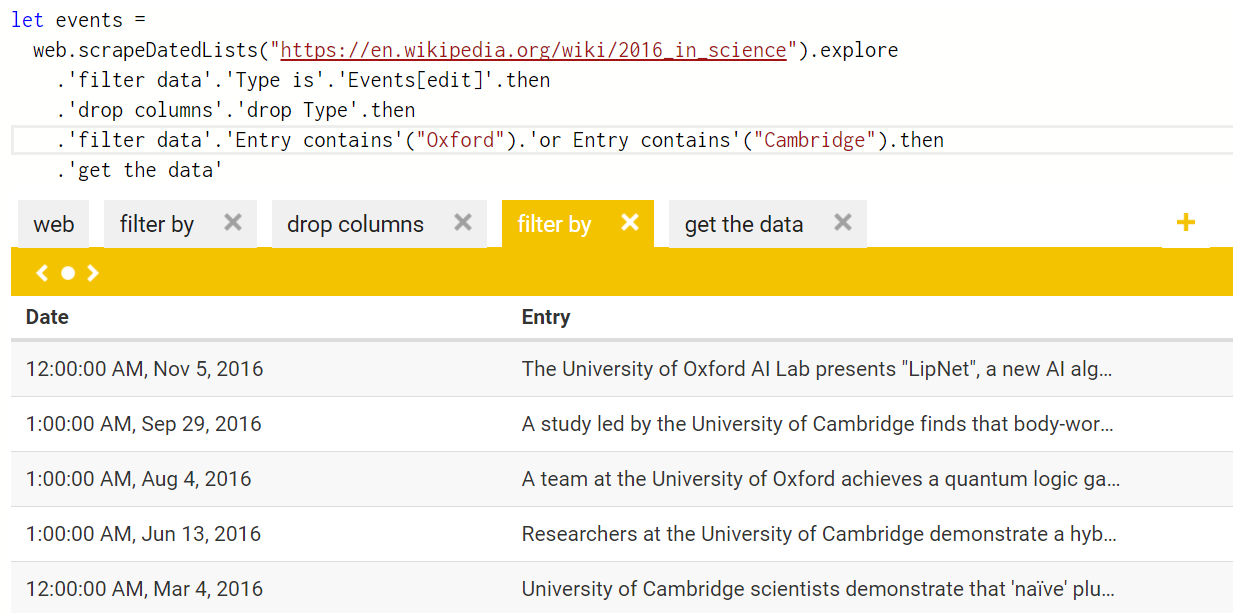
\includegraphics[scale=0.45]{scrape.png}
\caption{xxx}  
\end{figure*}

\newpage

% ==================================================================================================

\section{Live programming for data exploration}

The Gamma introduction and what this tries to do. See pretty screenshot.

This is what we care about - it's not live programming for your typical haskell,
but for R or Python.

\newpage
~

% ==================================================================================================

\begin{figure*}
\begin{equation*}
\begin{array}{l}
\xymatrix{
& \bnd{val}(\num{10}) &\qquad\quad& \bnd{val}(\num{15})\\
\bnd{var}(\ident{data}) & 
  \bnd{mem}(\ident{skip},s_0)\ar[l]_{\blbl{arg}(0)} \ar[u]^{\blbl{arg}(1)} && 
  \bnd{mem}(\ident{take},s_1)\ar[ll]_{\blbl{arg}(0)} \ar[u]_{\blbl{arg}(1)}
}\\[5em]
\xymatrix{
&& \bnd{val}(\num{10})\\
\bnd{var}(\ident{data}) & 
  \bnd{mem}(\ident{skip}, s_0)\ar[l]_{\blbl{arg}(0)} \ar@/^/[ru]^{\blbl{arg}(1)} && 
  \bnd{mem}(\ident{take}, s_2)\ar[ll]_{\blbl{arg}(0)} \ar@/_/[lu]_{\blbl{arg}(1)}
}
\end{array}\qquad
\begin{array}{l}
\textnormal{a.) The first graph is constructed from}\\
\textnormal{the following initial expression:}\\[0.5em]
\quad\kvd{let}~x = \num{15}~\kvd{in}\\
\quad\ident{data.skip}(\num{10}).\ident{take}(x)\\
\\
\textnormal{b.) The second diagram shows the updated graph}\\
\textnormal{after the programmer changes $x$ to $10$:}\\[0.5em]
\quad\kvd{let}~x = \num{10}~\kvd{in}\\
\quad\ident{data.skip}(\num{10}).\ident{take}(x)
\end{array}
\end{equation*}
\caption{Dependency graphs formed by two steps of the live programming process. }
\label{fig:dep-graph}
\end{figure*}

% --------------------------------------------------------------------------------------------------

\newpage


\section{Formalising live coding environment}
\label{sec:formal}

In this section, we present a formalisation of a live coding environment for a small,
expression-based programming language that supports \kvd{let} binding, member invocations
and $\lambda$ abstractions. This is the necessary minimum for data exploration as described
in the previous section.  

It excludes constructs such as a mechanism for defining new objects as we assume that those
are imported from the context through a mechanims such as type providers.
%
\begin{equation*}
\begin{array}{lcl}
e &=& \kvd{let}~x = e~\kvd{in}~e ~|~ \lambda x\rightarrow e ~|~ e.m(e, \ldots, e) ~|~ x ~|~ n
\end{array}
\end{equation*}
%
Here, $m$ ranges over member names, $x$ over variables and $n$ over primitive values such as 
numbers. Function values can be passed as arguments to methods (provided by a type provider), but 
for the purpose of this paper, we do not need to be able to invoke them directly.

\paragraph{The problem with functions.}
In the context of live programming, \kvd{let} binding and member access are unproblematic.
We can evaluate them and provide live preview for both of them, including all their sub-expressions.
Function values are more problematic, because their sub-expressions cannot be evaluated. For example:
%
\begin{equation*}
\begin{array}{l}
\kvd{let}~\ident{page} = \lambda x \rightarrow \ident{movies}.\ident{skip}(x*\num{10}).\ident{take}(\num{10})
\end{array}
\end{equation*}
%
We can provide live preview for the \ident{movies} sub-expression, but not for 
$\ident{movies}.\ident{skip}(x*\num{10})$ because we cannot obtain the value of $x$ without
running the rest of the program and analysing how the function is called later.

The method described in this paper does not provide live preview for sub-expressions that
contain free variables (which are not global objects provided by a type provider), but we
describe possible ways of doing so in Section~X and more speculative design of live coding 
friendly fucntions in Section~Y.

% --------------------------------------------------------------------------------------------------

\subsection{Maintaining dependency graph}
\label{sec:formal-deps}

The key idea behind our implementation is to maintain a dependency graph with nodes 
representing individual operations of the computation that can be partially evaluated
to obtain a preview. Each time the program text is modified, we parse it afresh (using an
error-recovering parser) and bind the abstract syntax tree to the dependency graph.

We remember the previously created nodes of the graph. When binding a new expression to
the graph, we reuse previously created nodes that have the same dependencies. For
expressions that have a new structure, we create new nodes (using a fresh symbol to 
identify them). 

The nodes of the graph serve as unique keys into a lookup table with previously
evaluated operations of the computation. When a preview is requested, we use the node
bound to the expression to find a preview, or evaluate it by first forcing the evaluation 
of all parents in the dependency graph.


% --------------------------------------------------------------------------------------------------

\begin{figure*}[t]
\vspace{-0.5em}
\begin{equation*}
\begin{array}{ll}
\ident{bind}_{\Gamma, \Delta}(e_0.m(e_1, \ldots, e_n)) = &(1)~~\\ 
\qquad \bndclr{v}, (\{\bndclr{v}\} \cup V_0 \cup \ldots \cup V_n, E \cup E_0 \cup \ldots \cup E_n)\\
\quad \textnormal{when}~\bndclr{v_i}, (V_i, E_i) = \ident{bind}_{\Gamma, \Delta}(e_i)\\
\quad \textnormal{and}~\bndclr{v} = \Delta(\bknd{mem}(m),[(\bndclr{v_0}, \blbl{arg}(0)), \ldots, (\bndclr{v_n}, \blbl{arg}(n))])\\
\quad \textnormal{let}~E = \{ (\bndclr{v}, \bndclr{v_0}, \blbl{arg}(0)), \ldots, (\bndclr{v}, \bndclr{v_n}, \blbl{arg}(n))\}
\\[0.75em]
\ident{bind}_{\Gamma, \Delta}(e_0.m(e_1, \ldots, e_n)) = &(2)\\ 
\qquad \bndclr{v}, (\{\bndclr{v}\} \cup V_0 \cup \ldots \cup V_n, E \cup E_0 \cup \ldots \cup E_n)\\
\quad \textnormal{when}~\bndclr{v_i}, (V_i, E_i) = \ident{bind}_{\Gamma, \Delta}(e_i)\\
\quad \textnormal{and}~(\bknd{mem}(m),[(\bndclr{v_0}, \blbl{arg}(0)), \ldots, (\bndclr{v_n}, \blbl{arg}(n))]) \notin \ident{dom}(\Delta)\hspace{-200em}.\\
\quad \textnormal{let}~\bndclr{v} = \bnd{mem}(m, s), s~\textnormal{fresh}\\
\quad \textnormal{let}~E = \{ (\bndclr{v}, \bndclr{v_0}, \blbl{arg}(0)), \ldots, (\bndclr{v},\bndclr{v_n}, \blbl{arg}(n)) \}
\\[0.75em]
\ident{bind}_{\Gamma, \Delta}(\kvd{let}~x=e_1~\kvd{in}~e_2) = \bndclr{v}, (\{\bndclr{v}\} \cup V \cup V_1, E \cup E_1)&(3)\\
\quad \textnormal{let}~\bndclr{v_1}, (V_1,E_1) = \ident{bind}_{\Gamma,\Delta}(e_1)\\
\quad \textnormal{let}~\Gamma_1 = \Gamma \cup \{(x,\bndclr{v_1})\} \\
\quad \textnormal{let}~\bndclr{v}, (V, E) = \ident{bind}_{\Gamma_1, \Delta}(e_2)
\end{array}
\begin{array}{ll}
\ident{bind}_{\Gamma, \Delta}(n) = \bnd{val}(n), (\{ \bnd{val}(n) \}, \emptyset) }&(4)
\\[0.75em]
\ident{bind}_{\Gamma, \Delta}(x) = \bndclr{v}, (\{ \bndclr{v} \}, \emptyset)\quad \textnormal{when}~\bndclr{v} = \Gamma(x)&(6)
\\[1em]
\ident{bind}_{\Gamma, \Delta}(\lambda x \rightarrow e) = \bndclr{v}, (\{\bndclr{v}\} \cup V, \{e\} \cup E)&(7)\\
\quad \textnormal{when}~\Gamma_1 = \Gamma \cup \{ x, \bnd{var}(x) \}\\
\quad \textnormal{and}~\bndclr{v_0}, (V, E) = \ident{bind}_{\Gamma_1, \Delta}(e)\\
\quad \textnormal{and}~\bndclr{v} = \Delta(\bknd{fun}(x),[(\bndclr{v_0}, \blbl{body})])\\
\quad \textnormal{let}~e = (\bndclr{v}, \bndclr{v_0}, \blbl{body}) 
\\[1em]
\ident{bind}_{\Gamma, \Delta}(\lambda x \rightarrow e) = \bndclr{v}, (\{\bndclr{v}\} \cup V, \{e\} \cup E)&(8)\\
\quad \textnormal{when}~\Gamma_1 = \Gamma \cup \{ x, \bnd{var}(x) \}\\
\quad \textnormal{and}~\bndclr{v_0}, (V, E) = \ident{bind}_{\Gamma_1, \Delta}(e)\\
\quad \textnormal{and}~(\bknd{fun}(x),[(\bndclr{v_0}, \blbl{body})])\notin \ident{dom}(\Delta)\\
\quad \textnormal{let}~\bndclr{v} = \bnd{fun}(s, x), s~\textnormal{fresh}\\
\quad \textnormal{let}~e = (\bndclr{v},\bndclr{v_0},\blbl{body}) 
\\[0.5em]
\end{array}
\end{equation*}
\vspace{-0.5em}
\caption{Rules of the binding process, which constructs a dependency graph for an expression.}
\label{fig:binding-rules}
\end{figure*}

% --------------------------------------------------------------------------------------------------
\paragraph{Elements of the graph.} The nodes of the graph represent individual operations
to be computed. In our design, the nodes themselves are used as keys, so we attach a unique 
\emph{symbol} to some of the nodes. That way, we can create two unique nodes representing, 
for example, access to a member named \ident{take} which differ in their dependencies.

Furthermore, the graph edges are labelled with labels indicating the kind of dependency. For
a method call, the labels are ``first argument'', ``second argument'' and so on. Formally:
%
\begin{equation*}
\begin{array}{rcll}
s&\hspace{-0.25em}\in\hspace{-0.25em}& \textit{Symbol}\\
i&\hspace{-0.25em}\in\hspace{-0.25em}& \textit{Integer}\\
n&\hspace{-0.25em}\in\hspace{-0.25em}& \textit{Primitive values}\\
x&\hspace{-0.25em}\in\hspace{-0.25em}& \textit{Variable names}\\
m&\hspace{-0.25em}\in\hspace{-0.25em}& \textit{Member names}\\[0.5em]
\bndclr{v}&\hspace{-0.25em}\in\hspace{-0.25em}&\bnd{val}(n)~|~\bnd{var}(x)~|~\bnd{mem}(m, s)~|~\bnd{fun}(x, s)&(\textit{Vertices})\\
\blblclr{l}&\hspace{-0.25em}\in\hspace{-0.25em}&\blbl{body}~|~\blbl{arg}(i)&(\textit{Edge labels})\\
\end{array}
\end{equation*}
%
The \bnd{val} node represents a primitive value and contains the value itself. Two occurences
of $\num{10}$ in the source code will be represented by the same node. Member access \bnd{mem}
contains the member name, together with a unique symbol -- two member access nodes with different 
dependencies will contain a different symbol. Dependencies of member access are labelled with 
\blbl{arg} indicating the index of the argument (the instance has index $0$ and arguments 
start with $1$).

Finally, nodes \bnd{fun} and \bnd{var} represent function values and variables bound by $\lambda$ 
abstraction. For simplicity, we use variable names rather than de Bruijn indices and so 
renaming a bound variable foces recomputation.

\paragraph{Example graph.} Figure~\ref{fig:dep-graph} illustrates how we construct and update the 
dependency graph. Node representing $\ident{take}(x)$ depends on the argument -- the
number $\num{15}$ -- and the instance, which is a node representing $\ident{skip}(\num{10})$.
This, in turn, depends on the instance \ident{data} and the number $\num{10}$. Note that variables
bound via \kvd{let} binding such as $x$ do not appear as $\bnd{var}$ nodes. The node using it
depends directly on the node representing the result of the expression that is assigned to $x$.

After changing the value of $x$, we create a new graph. The dependencies of the node 
$\bnd{mem}(\ident{skip}, s_0)$ are unchanged and so the node is reused. This means that this
part of the program is not recomputed. The $\blbl{arg}(1)$ dependency of the \ident{take} call 
changed and so we create a node $\bnd{mem}(\ident{skip}, s_2)$ with a new fresh symbol $s_2$.
The preview for this node is then recomputed as needed using the already known values of its
dependencies.

% --------------------------------------------------------------------------------------------------

\paragraph{Reusing graph nodes.} The binding process takes an expression and constructs a 
dependency graph, reusing existing nodes when possible. For this, we keep a lookup table 
of member access and function value nodes. The key is formed by a node kind (for 
disambiguation) together with a list of dependencies. A node kind is a member access or a function:
%
\begin{equation*}
\begin{array}{lcll}
\bkndclr{k}&\in&\bknd{fun}(x)~|~\bknd{mem}(m)&\qquad(\textit{Node  kinds})
\end{array}
\end{equation*}
%
Given a lookup table $\Delta$, we write $\Delta(\bkndclr{k}, [(\bndclr{n_1},\blblclr{l_1}), \ldots,
(\bndclr{v_n},\blblclr{l_n})])$ to perform a lookup for a node of a kind $\bkndclr{k}$ that has dependencies
$\bndclr{v_1}, \ldots, \bndclr{v_n}$ labelled with labels $\blblclr{l_1}, \ldots, \blblclr{l_n}$.

For example, when creating the graph in Figure~\ref{fig:dep-graph} (b), we perform the following
lookup for the \ident{skip} member access:
%
\[ \Delta(\bknd{mem}(\ident{skip}), [(\bnd{var}(\ident{data}),\blbl{arg}(0)), (\bnd{val}(\num{10}), \blbl{arg}(1))]) \]
%
The lookup returns the node $\bnd{mem}(\ident{skip}, s_0)$ known from the previous step. We then perform
the following lookup for the \ident{take} member access:
%
\[ \Delta(\bknd{mem}(\ident{take}), [(\bnd{mem}(\ident{skip}, s_0),\blbl{arg}(0)), (\bnd{val}(\num{10}), \blbl{arg}(1))]) \]
%
In the previous graph, the argument of \ident{take} was $\num{15}$ rather than $\num{10}$ and so
this lookup fails. We then construct a new node $\bnd{mem}(\ident{take}, s_2)$ using a fresh
symbol $s_2$.

% --------------------------------------------------------------------------------------------------

\subsection{Binding an expressions to a graph}
\label{sec:formal-bind}

When constructing the dependency graph, our implementation annotates the nodes of the 
abstract syntax tree with the nodes of the dependency graph, forming a mapping
$e \rightarrow \bndclr{v}$. For this reason, we call the process \emph{binding}.

The process of binding is defined by the rules in Figure~\ref{fig:binding-rules}.
The \ident{bind} function is annotated with a lookup table $\Delta$ discussed in 
Section~\ref{sec:formal-deps} and a variable context $\Gamma$. The variable context 
is a map from variable names to dependency graph nodes and is used for variables bound
using \kvd{let} binding.

When applied on an expression $e$, binding $\ident{bind}_{\Gamma,\Delta}(e)$ returns a
dependency graph $(V, E)$ paired with a node $\bndclr{v}$ corresponding to the expression $e$.
In the graph, $V$ is a set of nodes $\bndclr{v}$ and $E$ is a set of labelled edges
$(\bndclr{v_1}, \bndclr{v_2}, \blblclr{l})$. We attach the label directly to the edge rather than
keeping a separate colouring function as this makes the formalisation simpler.

\paragraph{Binding member access.} In all rules, we recursively bind sub-expressions to get
a dependency graph for each sub-expression and a graph node that represents it. The nodes 
representing sub-expressions are then used as dependencies for lookup into $\Delta$, together
with their labels. When binding a member access, we reuse an existing node if it is defined by 
$\Delta$ (1) or we create a new node containing a fresh symbol when the domain of $\Delta$ does 
not contain a key describing the current member access~(2). 

\paragraph{Binding let binding.} For \kvd{let} binding (3), we first bind the expression $e_1$ assigned
to the variable to obtain a graph node $\bndclr{v_1}$. We then bind the body expression $e_2$,
but using a variable context $\Gamma_1$ that maps the value of the variable to the graph node
$\bndclr{v_1}$. The variable context is used when binding a variable (6) and so all variables 
declared using \kvd{let} binding will be bound to a graph node representing the value assinged 
to the variable. The node bound to the overall \kvd{let} expression is then the graph node bound
to the body expression.

\paragraph{Binding function values.} If a function value uses its argument, we will not be able
to evaluate its body. In this case, the graph node bound to a function will depend on a synthetic
node $\bnd{var}(x)$ that represents the variable with no value. When binding a function, we 
create the synthetic variable and add it to the variable context $\Gamma_1$ before binding the
body. As with member access, the node representing a function may (7) or may not (8) be already 
present in the lookup table.

% --------------------------------------------------------------------------------------------------

\begin{figure}[!b]
\vspace{-0.5em}
\begin{equation*}
\begin{array}{l}
\Delta_{i}(\bknd{mem}(m), [(\bndclr{v_0},\blbl{arg}(0)),\ldots, (\bndclr{v_n},\blbl{arg}(n))]) = \bndclr{v}\\
\quad \textnormal{for all}~\bnd{mem}(m, s) \in V\\
\quad \textnormal{such that}~(\bnd{mem}(m, s), \bndclr{v_i}, \blbl{arg}(i)) \in E~\textnormal{for}~i\in 0,..,n
\\[0.75em]
\Delta_{i}(\bknd{fun}(x), [(\bndclr{v_1},\blbl{body})]) = \bndclr{v}\\
\quad \textnormal{for all}~\bnd{fun}(x, s) \in V\\
\quad \textnormal{such that}~(\bnd{fun}(x, s), \bndclr{v_1}, \blbl{body}) \in E
\\[0.75em]
\Delta_{i}(\bkndclr{v}) = \Delta_{i-1}(\bkndclr{v})\quad \textnormal{(otherwise)}
\end{array}
\end{equation*}
\vspace{-0.5em}
\caption{Updating the node cache after binding a new graph}
\label{fig:loop}
\end{figure}

% --------------------------------------------------------------------------------------------------

\begin{figure*}
\begin{equation*}
\qquad\qquad\quad\begin{array}{l}
\inference[(lift-expr)~]
  {\bndclr{v} \Downarrow \llbracket e \rrbracket_\Gamma}
  {\bndclr{v} \Downarrow_{\ident{lift}} \llbracket e \rrbracket_\Gamma}
\\
\\
\inference[(lift-prev)~]
  {\bndclr{v} \Downarrow p}
  {\bndclr{v} \Downarrow_{\ident{lift}} \llbracket p \rrbracket_\emptyset}
\\
\\
\inference[(val)~]
  {~}
  {\bnd{val}(n) \Downarrow n }
\\
\\
\inference[(var)~]
  {~}
  {\bnd{var}(x) \Downarrow \llbracket x \rrbracket_x}
  \\[0.5em]~
\end{array}
\qquad
\begin{array}{l}
\inference[(fun-val)~]
  { (\bnd{fun}(x, s), \bndclr{v}, \blbl{body}) \in E & \bndclr{v} \Downarrow p }
  { \bnd{fun}(x, s) \Downarrow \lambda x\rightarrow p }
\\
\\
\inference[(fun-bind)~]
  { (\bnd{fun}(x, s), \bndclr{v}, \blbl{body}) \in E & \bndclr{v} \Downarrow \llbracket e \rrbracket_{x} }
  { \bnd{fun}(x, s) \Downarrow \lambda x\rightarrow e }
\\
\\
\inference[(fun-expr)~]
  { (\bnd{fun}(x, s), \bndclr{v}, \blbl{body}) \in E & \bndclr{v} \Downarrow \llbracket e \rrbracket_{x,\Gamma} }
  { \bnd{fun}(x, s) \Downarrow \llbracket \lambda x\rightarrow e \rrbracket_\Gamma }
\\[0.5em]~
\end{array}
\end{equation*}
\begin{equation*}  
\qquad\qquad\begin{array}{l}
\inference[(mem-val)~]
  { \forall i\in\{0\ldots k\}.(\bnd{mem}(m, s), \bndclr{v_i}, \blbl{arg}(i)) \in E & \bndclr{v_i} \Downarrow p_i 
    & p_0.m(p_1, \ldots, p_k) \rightsquigarrow p }
  { \bnd{mem}(m, s) \Downarrow p }
\\  
\\
\inference[(mem-expr)~]
  { \forall i\in\{0\ldots k\}.(\bnd{mem}(m, s), \bndclr{v_i}, \blbl{arg}(i)) \in E & \exists j\in\{0\ldots k\}.\bndclr{v_j}\diagup\hspace{-1em}\Downarrow p_j
   & \bndclr{v_i} \Downarrow_{\ident{lift}} \llbracket e_i \rrbracket_{\Gamma_i}  }
  { \bnd{mem}(m, s) \Downarrow \llbracket e_0.m(e_1, \ldots, e_k) \rrbracket_{\Gamma_0,\ldots,\Gamma k} }
\\
\end{array}
\end{equation*}

\caption{Rules that define evaluation of previews over a dependency graph for an expression}  
\label{fig:eval}
\end{figure*}

% --------------------------------------------------------------------------------------------------


\subsection{Edit and rebind loop}

The binding process formalised in Section~\ref{sec:formal-bind} specifies how to update the 
dependency graph after updated program text is parsed. During live coding, this is done 
repeatedly as the programmer edits code. Throughout the process, we maintain a series of 
lookup table states $\Delta_0, \Delta_1, \Delta_2, \ldots$. Initially, the lookup table is 
empty, i.e.~$\Delta_0 = \emptyset$.

At a step $i$, we parse an expression $e_i$ and calculate the new dependency graph and a node
bound to the top-level expression using the previous $\Delta$:
%
\begin{equation*}
\bndclr{v}, (V, E) = \ident{bind}_{\emptyset, \Delta_{i-1}}(e_i)
\end{equation*}
%
The new state of the node cache is then computed by adding newly created nodes from the graph
$(V, E)$ to the previous cache $\Delta_{i-1}$. This is done for function and member nodes that
contain unique symbols as defined in Figure~\ref{fig:loop}. We do not need to cache nodes
representing primitive values and variables as those do not contain symbols and will remain the
same due to the way they are constructed.

% ==================================================================================================

\section{Evaluating previews}
\label{sec:previews}

The mechanism for constructing dependency graphs defined in Section~\ref{sec:formal} makes it
possible to provide live previews when editing code without recomputing the whole program 
each time the source code changes.

The nodes in the dependency graph correspond to individual operations that will be performed
when running the program. When the dependencies of an operation do not change while editing 
code, the subsequent dependency graph will reuse a node used to represent the operation. 

Our live editor keeps a map from graph nodes to live previews, so a new preview only needs to be
computed when a new node appears in the dependency graph (and the user moves the cursor to a 
code location that corresponds to the node). This section describes how previews are evaluated.

\paragraph{Previews and delayed previews.}
As discussed in Section~\ref{sec:formal}, the body of a function cannot be easily evaluated to
a value if it uses the bound variable. We do not attempt to ``guess'' possible arguments and,
instead, provide a full preview only for sub-expressions with free variables bound by a let binding.
For a function body that uses the bound variable, we obtain a \emph{delayed preview}, which is
an expression annotated with a list of variables that need to be provided before the expression
can be evaluated. We use the following notation:
%
\begin{equation*}
\begin{array}{rcll}
p&\hspace{-0.25em}\in\hspace{-0.25em}&n~|~\lambda x\rightarrow e&\quad(\textit{Fully evaluated previews})\\
d&\hspace{-0.25em}\in\hspace{-0.25em}&p~|~\llbracket e \rrbracket_\Gamma&\quad(\textit{Evaluated and delayed previews})\\
\end{array}
\end{equation*}
%
Here, $p$ ranges over fully evaluated values. It can be either a primitive value (such as number,
string or an object) or a function value with no free variables. A possibly delayed preview $d$ 
can then be either evaluated preview $p$ or an expression $e$ that requires variables $\Gamma$.
For simplicity, we use an untyped language and so $\Gamma$ is a list of variables $x_1, \ldots, x_n$.

\paragraph{Evaluation and splicing.}
In this paper, we omit the specifics of the underlying programming langauge and we focus on the
live coding mechanism. However, we assume that the language is equipped with an evaluation 
reduction $e \rightsquigarrow p$ that reduces a closed expression $e$ into a value $p$.

For delayed previews, we construct a delayed expression using splicing. For example, assuming
we have a delayed previews $\llbracket e_0 \rrbracket_x$ and $\llbracket e_1 \rrbracket_y$. 
If we need to invoke a member $m$ on $e_0$ using $e_1$ as an argument, we construct a new 
delayed preview $\llbracket e_0.m(e_1) \rrbracket_{x, y}$. This operation is akin to expression
splicing from meta-programming [X,Y] and can be more formally captured by Contextual Modal Type 
Theory (CMTT) as outlined below.

\paragraph{Evaluation of previews.}
The evaluation of previews is defined in Figure~\ref{fig:eval}. Given a dependency graph $(V, E)$,
we define a relation $\bndclr{v}\Downarrow d$ that evaluates a sub-expression corresponding to 
the node $\bndclr{v}$ to a (possibly delayed) preview $d$. 

The auxiliary relation $\bndclr{v}\Downarrow_{\ident{lift}} d$ always evaluates
to a delayed preview. If the ordinary evaluation returns a delayed preview, so does the auxiliary
relation (\emph{lift-expr}). If the ordinary evaluation returns a value, the value is wrapped
into a delayed preview requiring no variables (\emph{lift-prev}).

Graph node representing a value is evaluated to a value (\emph{val}) and a graph node representing
an unbound variable is reduced to a delayed preview that requires the variable and returns its
value (\emph{var}).

For member access, we distinguish two cases. If all arguments evaluate to values (\emph{member-val}),
then we use the evaluation relation $\rightsquigarrow$, immediately evaluate the member access and 
produce a value. If one of the arguments is delayed (\emph{member-expr}), because the member access 
is in the body of a lambda function, then we produce a delayed member access experession that
requires the union of the variables required by the individual arguments.

Finally, the evaluation of function values is similar, but requires three cases. If the body can 
be reduced to a value with no unbound variables (\emph{fun-val}), we return a lambda function that
returns the value. If the body requires only the bound variable (\emph{fun-bind}), we return a 
lambda function with the delayed preview as the body. If the body requires further variables,
the result is a delayed preview containing a function.

\paragraph{Caching previews.}
For simplicity, the relation $\Downarrow$ in Figure~\ref{fig:eval} does not specify how previews 
are cached and linked to graph nodes. In practice, this is done by maintaining a lookup table
$\bndclr{v} \rightarrow p$ from graph nodes $\bdnclr{v}$ to (possibly delayed) previews $p$.
Whenever the $\Downarrow$ relation is used to obtain a preview for a graph node, we first 
attempt to find an already evaluated preview using the lookup table. If the preview has not
been previously evaluated, we evaluate it and add it to the lookup table.

This means that evaluated previews can be reused in two ways. First, multiple nodes can 
depend on one sub-graph in a single dependency graph (e.g.~if the same sub-expression appears
twice in the program). Second, the keys of the lookup table are graph nodes and nodes are 
reused when a new dependency graph is constructed after the user edits the source code.

\paragraph{Semantics of delayed previews.}
The focus of this paper is on the design and implementation of a live coding environment, 
but it is worth noting that the structure of delayed previews is closely linked to the work
on Contextual Modal Type Theory (CMTT) [X] and comonads [Y]. 

In CMTT, $\lbrack \Psi \rbrack A$ denotes that a proposition $A$ is valid in context $\Psi$,
which is closely related to our delayed preivews written as $\llbracket A \rrbracket_\Psi$.
CMTT defines rules for composing context-dependent propositions that would allow us to express
the splicing operation used in (\emph{mem-expr}). In categorical terms, the context-dependent
proposition can be modelled as an indexed comonad [X]. The evaluation of a preview with no 
context dependencies (built implicitly into our evaluation rules) corresponds to the counit
operation of a comonad and would be explicitly written as $\llbracket A \rrbracket_\emptyset \rightarrow A$.

% ==================================================================================================

\section{Properties}
\newpage

Something about how dependency graph bits are reused correctly, i.e. if there is a source code
change that can change the result, the graph will change.

Something about various code edit operations that will not cause recomputation.

% --------------------------------------------------------------------------------------------------

\newpage

\newpage

\section*{References}

\bibliography{paper}

\end{document}
